\documentclass[aspectratio=43]{beamer}
\usepackage[utf8]{inputenc}
\usepackage[english,russian]{babel}
\usepackage[T2A]{fontenc}


\sloppy

\newcommand{\lama}{$\lambda\kern -.1667em\lower -.5ex\hbox{$a$}\kern -.1000em\lower .2ex\hbox{$\mathcal M$}\kern -.1000em\lower -.5ex\hbox{$a$}$\xspace}

\mode<presentation>{
  \usetheme{IPLC}
}

\begin{document}

\begin{frame}[fragile]{Языки программирования}
  \onslide<2->{
  \begin{columns}
  \column{0.6\textwidth}
  \begin{itemize}      
  \item Синтаксис
    \onslide<3->{\begin{itemize}\item Форма представления программ\end{itemize}}
  \item Семантика
    \onslide<4->{\begin{itemize}\item ``Смысл'' программ\end{itemize}}
  \item Прагматика
    \onslide<5->{\begin{itemize}\item Взаимодействие языка программирования с программистом\end{itemize}}
  \end{itemize}
\column{0.4\textwidth}
\begin{figure}
  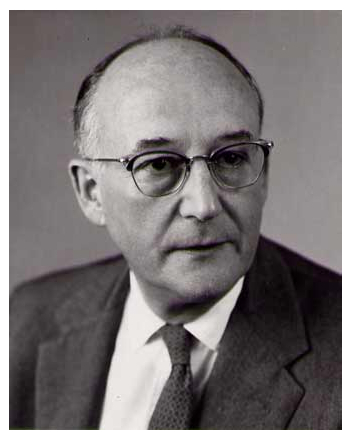
\includegraphics[scale=0.25]{images/morris.jpg}
  \caption{Чарльз Уильям Моррис (1903-1979)}
 \end{figure}
\end{columns}}  
\end{frame}

\begin{frame}[fragile]{Синтаксис}
  \newsavebox{\mybox}
  \begin{lrbox}{\mybox}
    \begin{tikzpicture}
    \node (main) at (0, 0) {
    \begin{lstlisting}[basicstyle=\fontencoding{T1}\footnotesize\fontfamily{lmtt}\fontseries{c}\selectfont,morekeywords={if,else},keywordstyle=\underline]
    if (n > 100) n = 10; else f (f (n + 11));
    \end{lstlisting}};
    \onslide<3->{
    \node at (-3.5, 0.5) {\textit{\textsf{\tiny{ключевое слово}}}};
    \node at (-0.3, 0.4) {\textit{\textsf{\tiny{десятичная константа}}}};
    \node at (-2.8, 0.9) {\textit{\textsf{\tiny{разделитель}}}};
    \node at (-2.5, 1.2) {\textit{\textsf{\tiny{идентификатор}}}};
    \node at (-1.5, 0.7) {\textit{\textsf{\tiny{бинарная операция}}}};
    \draw[-stealth] (-3.4,  0.4) -- (-3.4, 0.2);
    \draw[-stealth] (-2.7,  0.8) -- (-2.7, 0.2);
    \draw[-stealth] (-2.9,  1.1) -- (-2.9, 0.2);
    \draw[-stealth] (-2.3,  0.6) -- (-2.3, 0.2);
    \draw[-stealth] (-1.6, 0.42) -- (-1.8, 0.42) -- (-1.8, 0.2);
    }
    \onslide<4->{
    \node at (0    ,   -1) {\textit{\textsf{\tiny{оператор}}}};
    \node at (-0.35, -0.5) {\textit{\textsf{\tiny{оператор}}}};
    \node at (3    , -0.5) {\textit{\textsf{\tiny{оператор}}}};
    \node at (-2.1 , -0.5) {\textit{\textsf{\tiny{выражение}}}};
    \draw [decorate,decoration = {brace,mirror}] (-3.5, -0.7) -- (4.2, -0.7);    
    \draw [decorate,decoration = {brace,mirror}] (-2.9, -0.2) -- (-1.3, -0.2);    
    \draw [decorate,decoration = {brace,mirror}] (-1, -0.2) -- (0.3, -0.2);    
    \draw [decorate,decoration = {brace,mirror}] (1.6, -0.2) -- (4.2, -0.2);
    }
    \end{tikzpicture}
  \end{lrbox}
  \begin{itemize}
  \item Лексический и грамматический уровень
      \onslide<2->{
      \usebox{\mybox}
      \global\let\mybox\relax}
    \item Однозначность
          \onslide<5->{
    \begin{itemize}\item ``Входя в двери лифта с животными,\\ придерживайте их.''\end{itemize}}
  \item Эффективная распознаваемость
  \end{itemize}  
\end{frame}

\begin{frame}[fragile]{Семантика}
  \newsavebox{\mybox}
  \begin{lrbox}{\mybox}
    \begin{lstlisting}[basicstyle=\fontencoding{T1}\footnotesize\fontfamily{lmtt}\fontseries{c}\selectfont,morekeywords={if,else},keywordstyle=\underline]
      0*(x/0) = ?
      -x+1+x  = ?
      x+1-1   = ?
    \end{lstlisting}
  \end{lrbox}
  \begin{itemize}
  \item Неформальная семантика
    \onslide<2->{
      \begin{itemize}\item ``Выражения состоят из переменных, констант и знаков четырех арифметических действий'' \end{itemize}
      \onslide<3->{\usebox{\mybox}\global\let\mybox\relax}}
      \onslide<4->{\begin{itemize}\item Примеры ``запутанных'' программ: \footnotesize\fontfamily{lmtt}\fontseries{c}\selectfont{https://www.cise.ufl.edu/\textasciitilde manuel/obfuscate/obfuscate.html}\end{itemize}}
  \item Формальная семантика
    \onslide<5->{\begin{itemize}\item Специальная математическая теория\end{itemize}}
  \end{itemize}  
\end{frame}

\begin{frame}[fragile]{Трансляция}
  \begin{itemize}
  \item Синтаксическое преобразование программы на одном языке в программу на другом
    \vskip1cm
    \begin{figure}
    \begin{tikzpicture}[node distance = 2cm,auto,font=\footnotesize,
% STYLES
every node/.style={node distance=1cm},
% The comment style is used to describe the characteristics of each force
comment/.style={rectangle, inner sep= 5pt, text width=8cm, node distance=1cm, font=\scriptsize\sffamily},
% The force style is used to draw the forces' name
pgm/.style={tape, draw, inner sep=5pt, font=\it\scriptsize\sffamily},
trn/.style={circle, draw, inner sep=5pt, font=\it\scriptsize\sffamily}
      ]
      \node (trn) [trn] {Транслятор};
      \node (src) [pgm, left=of trn, minimum height=1.5cm] {Программа};
      \node (tag) [pgm, right=of trn, minimum height=1.5cm] {Программа};
      
      \draw [-stealth] (src) -- (trn);      
      \draw [-stealth] (trn) -- (tag);
      
      \onslide<2->{
        \node (srcLan) [below=of src] {\textit{\textsf{\tiny{\begin{tabular}{c}
                                                                исходный язык\\
                                                                (source language)
                                                             \end{tabular}
                                      }}}};
        \draw [-stealth] (srcLan) -- (src);
       }

      \onslide<3->{
        \node (tagLan) [below=of tag] {\textit{\textsf{\tiny{\begin{tabular}{c}
                                                                целевой язык\\
                                                                (target language)
                                                             \end{tabular}
                                      }}}};
        \draw [-stealth] (tagLan) -- (tag);
      }

      \onslide<4->{
        \node (impLan) [below=of trn] {\textit{\textsf{\tiny{\begin{tabular}{c}
                                                                инструментальный язык\\
                                                                (implementation language)
                                                             \end{tabular}
                                      }}}};      
        \draw [-stealth] (impLan) -- (trn);
      }
    \end{tikzpicture}
    \end{figure}
   % \begin{itemize}
   %   \item Исходный язык: язык, с которого производится трансляция
   %   \item Целевой язык: язык, в который производится трансляция
   %   \item Инструментальный язык: язык реализации транслятора
   %  \end{itemize}
  \end{itemize}  
\end{frame}

\begin{frame}[fragile]{Виды трансляторов}
  \begin{center}
    Языки \emph{высокого} уровня \emph{vs.} языки \emph{низкого} уровня
  \end{center}  
  \begin{itemize}
    \item \onslide<2->{$\mbox{\emph{высокий}}\to\mbox{\emph{высокий}}$~--- конвертор}
    \item \onslide<3->{$\mbox{\emph{высокий}}\to\mbox{\emph{низкий}}$~--- компилятор}
    \item \onslide<4->{$\mbox{\emph{низкий}}\to\mbox{\emph{высокий}}$~--- декомпилятор}
    \item \onslide<5->{$\mbox{\emph{низкий}}\to\mbox{\emph{низкий}}$~--- бинарный транслятор}
  \end{itemize}
\end{frame}

\begin{frame}[fragile]{Окружение и кросс-компиляция}
  \begin{itemize}
  \onslide<2->{ 
  \item Окружение (\emph{environment}):
    \begin{itemize}
    \item аппаратная архитектура
    \item ОС
    \item библиотеки
    \end{itemize}
  }
  \onslide<3->{
  \item \emph{Инструментальное} окружение vs. \emph{целевое} окружение
  }
  \onslide<4->{
  \item \emph{Кросс}-компиляция (\emph{cross-compilation}):
    \begin{figure}
    \begin{tikzpicture}
      \node (impl)                     {
\includegraphics{images/supercomputer.jpg}};
      \node (target) [right=of impl]   {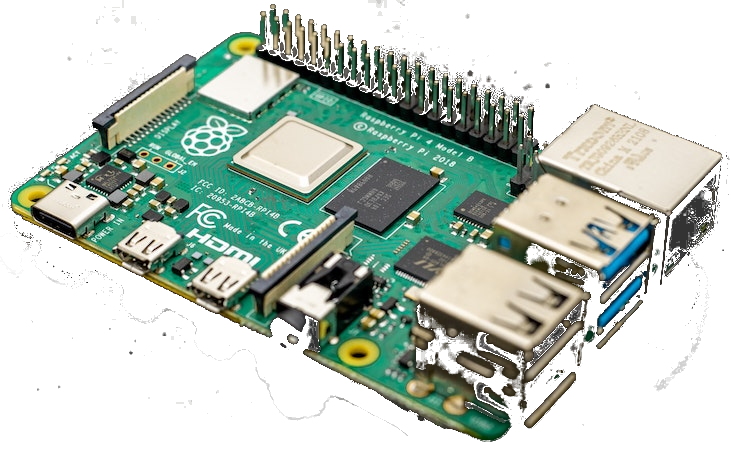
\includegraphics[scale=0.05]{images/raspberry.png}};
      \node (pad)    [right=of target] {};
      \draw [-stealth] (impl) -- (target);
    \end{tikzpicture}
    \end{figure}
  }
  \end{itemize}
\end{frame}

\begin{frame}[fragile]{Раскрутка (\emph{bootstrapping})}
  \begin{center}
       Язык реализации = исходный язык
    \begin{figure}
      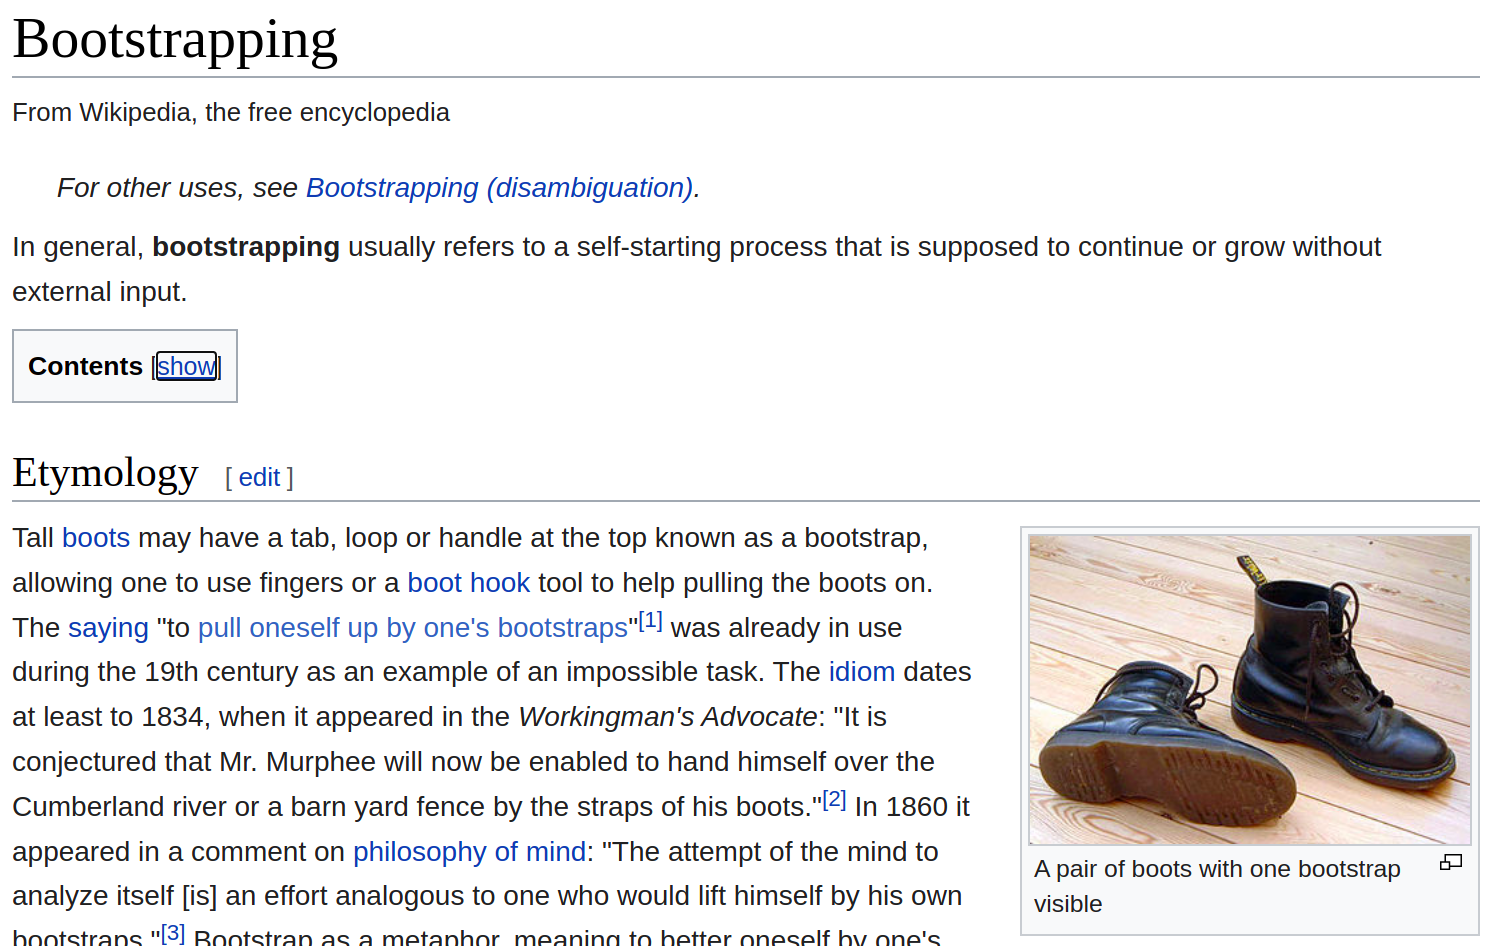
\includegraphics[scale=0.2]{images/bootstrapping.png}
    \end{figure}
  \end{center}
\end{frame}

\begin{frame}[fragile]{Полная \emph{vs.} частичная корректность}
  
  \begin{itemize}
    \onslide<2->{
    \item \emph{Полная} корректность:}
    \onslide<3->{
    \begin{figure}
      \begin{tikzpicture}
        \node (a-src-x)                    {x};
        \node (a-src-y) [right=of a-src-x] {y};
        \draw [-stealth] (a-src-x) -- node[above]{\scalebox{0.5}{исходная}} (a-src-y);
        
        \node (righta)  [right=of a-src-y,yshift=1mm] {$\xRightarrow{\phantom{XXX}}$};
        
        \node (a-tgt-x) [right=of righta,yshift=-1mm]  {x};
        \node (a-tgt-y) [right=of a-tgt-x] {y};
        \draw [-stealth] (a-tgt-x) -- node[above]{\scalebox{0.5}{целевая}}  (a-tgt-y);
      \end{tikzpicture}      
    \end{figure}}
    \onslide<4->{
    \begin{figure}
      \begin{tikzpicture}
        \node (a-src-x)                    {x};
        \node (a-src-y) [right=of a-src-x] {y};
        \draw [-stealth] (a-src-x) -- node[above]{\scalebox{0.5}{исходная}} (a-src-y);
        
        \node (righta)  [right=of a-src-y,yshift=1mm] {$\xLeftarrow{\phantom{XXX}}$};
        
        \node (a-tgt-x) [right=of righta,yshift=-1mm]  {x};
        \node (a-tgt-y) [right=of a-tgt-x] {y};
        \draw [-stealth] (a-tgt-x) -- node[above]{\scalebox{0.5}{целевая}}  (a-tgt-y);

        \onslide<5->{
          \draw [color=red] (0, -0.5) -- (7, 0.5);
          \draw [color=red] (0, 0.5) -- (7, -0.5);
        }
      \end{tikzpicture}      
    \end{figure}}
    \onslide<5->{
    \item \emph{Частичная} корректность
      \begin{tikzpicture}[overlay]
        \draw [-stealth] (-1.5, -0.3) .. controls (-0.8, -1) and (0, -1) .. (0.3, 0.5);
      \end{tikzpicture}
    }
  \end{itemize}
  
\end{frame}

\begin{frame}[fragile]{Архитектура компиляторов}
  \begin{itemize}
    \onslide<2->{
    \item Просмотры (\emph{passes})
    }
    \onslide<3->{
    \item Промежуточное представление (\emph{intermediate representation, IR})
    }
  \end{itemize}
  \begin{figure}
    \begin{tikzpicture}[node distance=0.5mm]
      \onslide<4-5>{
      \node                                                                                                  (pad)    {};
      \node [shape=rectangle,draw,rounded corners,below=of pad,minimum width=2.8cm,minimum height=0.45cm]    (syntax) {\scriptsize{\begin{tabular}{c}
                                                                                                                                        синтаксический\\
                                                                                                                                        анализ
                                                                                                                                    \end{tabular}}};
      \node [shape=rectangle,draw,rounded corners,below=of syntax,minimum width=2.8cm,minimum height=0.45cm] (types)  {\scriptsize{\begin{tabular}{c}
                                                                                                                                        анализ\\
                                                                                                                                        типов
                                                                                                                                    \end{tabular}}};
      \node [shape=rectangle,draw,rounded corners,below=of types,minimum width=2.8cm,minimum height=0.45cm]  (other)  {\scriptsize{...}};
      \begin{scope}
        \node[fit = (pad)(syntax)(types)(other),shape=rectangle,draw,rounded corners] (analysis) {};
      \end{scope}
      \node [shape=rectangle, fill=black,yshift=2.8mm] (analysis) {\scriptsize{\begin{tabular}{c}
                                                                                  Анализ \\
                                                                                (frontend)
                                                                               \end{tabular}}};
      }
      \onslide<5>{
      \node [right=3.7cm of pad]                                                                               (pads)    {};
      \node [shape=rectangle,draw,rounded corners,below=of pads,minimum width=2.6cm,minimum height=0.4cm]    (syntaxs) {\scriptsize{\begin{tabular}{c}
                                                                                                                                        выбор\\
                                                                                                                                        инструкций
                                                                                                                                    \end{tabular}}};
      \node [shape=rectangle,draw,rounded corners,below=of syntaxs,minimum width=2.6cm,minimum height=0.4cm] (typess)  {\scriptsize{\begin{tabular}{c}
                                                                                                                                         распределение\\
                                                                                                                                         регистров
                                                                                                                                    \end{tabular}}};
      \node [shape=rectangle,draw,rounded corners,below=of typess,minimum width=2.6cm,minimum height=0.4cm]  (others)  {\scriptsize{...}};
      \begin{scope}
        \node[fit = (pads)(syntaxs)(typess)(others),shape=rectangle,draw,rounded corners] (synthesis) {};
      \end{scope}
      \node [shape=rectangle, fill=black,yshift=2.8mm,xshift=3.9cm] (synthesis) {\scriptsize{\begin{tabular}{c}
                                                                                                   Синтез \\
                                                                                                  (backend)
                                                                                             \end{tabular}}};
      \draw [-stealth,thick] (1.7,-0.7) -- (2.4,-0.7);
      }
      \onslide<6>{
      \node                                                                                                 (pad)    {};
      \node [shape=rectangle,draw,rounded corners,below=of pad,minimum width=2.8cm,minimum height=0.45cm]    (syntax) {\scriptsize{\begin{tabular}{c}
                                                                                                                                        синтаксический\\
                                                                                                                                        анализ
                                                                                                                                    \end{tabular}}};
      \node [shape=rectangle,draw,rounded corners,below=of syntax,minimum width=2.8cm,minimum height=0.45cm] (types)  {\scriptsize{\begin{tabular}{c}
                                                                                                                                        анализ\\
                                                                                                                                        типов
                                                                                                                                    \end{tabular}}};
      \node [shape=rectangle,draw,rounded corners,below=of types,minimum width=2.8cm,minimum height=0.45cm]  (other)  {\scriptsize{...}};
      \begin{scope}
        \node[fit = (pad)(syntax)(types)(other),shape=rectangle,draw,rounded corners] (analysis) {};
      \end{scope}
      \node [shape=rectangle, fill=black,yshift=2.8mm] (analysis) {\scriptsize{\begin{tabular}{c}
                                                                                  Анализ \\
                                                                                (frontend)
                                                                               \end{tabular}}};


      \node [right=3.7cm of pad]                                                                               (pado)    {};
      \node [shape=rectangle,draw,rounded corners,below=of pado,minimum width=2.6cm,minimum height=0.4cm]    (syntaxo) {\scriptsize{\begin{tabular}{c}
                                                                                                                                        оптимизация\\
                                                                                                                                        переходов
                                                                                                                                    \end{tabular}}};
      \node [shape=rectangle,draw,rounded corners,below=of syntaxo,minimum width=2.6cm,minimum height=0.4cm] (typeso)  {\scriptsize{\begin{tabular}{c}
                                                                                                                                         устранение\\
                                                                                                                                         мертвого кода
                                                                                                                                    \end{tabular}}};
      \node [shape=rectangle,draw,rounded corners,below=of typeso,minimum width=2.6cm,minimum height=0.4cm]  (othero)  {\scriptsize{...}};
      \begin{scope}
        \node[fit = (pado)(syntaxo)(typeso)(othero),shape=rectangle,draw,rounded corners] (opt) {};
      \end{scope}
      \node [shape=rectangle, fill=black,yshift=2.8mm,xshift=3.9cm] (synthesis) {\scriptsize{\begin{tabular}{c}
                                                                                                   Оптимизация \\
                                                                                                  (middle-end)
                                                                                             \end{tabular}}};
      \draw [-stealth,thick] (1.7,-0.7) -- (2.4,-0.7);

      \node [right=7.7cm of pad]                                                                               (pads)    {};
      \node [shape=rectangle,draw,rounded corners,below=of pads,minimum width=2.6cm,minimum height=0.4cm]    (syntaxs) {\scriptsize{\begin{tabular}{c}
                                                                                                                                         выбор\\
                                                                                                                                         инструкций
                                                                                                                                    \end{tabular}}};
      \node [shape=rectangle,draw,rounded corners,below=of syntaxs,minimum width=2.6cm,minimum height=0.4cm] (typess)  {\scriptsize{\begin{tabular}{c}
                                                                                                                                         распределение\\
                                                                                                                                         регистров
                                                                                                                                    \end{tabular}}};
      \node [shape=rectangle,draw,rounded corners,below=of typess,minimum width=2.6cm,minimum height=0.4cm]  (others)  {\scriptsize{...}};
      \begin{scope}
        \node[fit = (pads)(syntaxs)(typess)(others),shape=rectangle,draw,rounded corners] (synthesis) {};
      \end{scope}
      \node [shape=rectangle, fill=black,yshift=2.8mm,xshift=7.9cm] (synthesis) {\scriptsize{\begin{tabular}{c}
                                                                                                   Синтез \\
                                                                                                  (backend)
                                                                                             \end{tabular}}};
      \draw [-stealth,thick] (5.65,-0.7) -- (6.35,-0.7);
      }
    \end{tikzpicture}
  \end{figure}
\end{frame}

\begin{frame}[fragile]{Компилятор \lama}
  x
\end{frame}

\end{document}
